%\subsection{PV hierarchy}\label{sec:back_pv:hierarcy}
A PV module is an assembly of photo-voltaic cells using solar irradiance as a source of energy to generate direct current electricity. A PV module is described by a {voltage-current (I-V) characteristic curve} (left of Figure~\ref{fig:moduleStructure}, black lines), which changes as a function of the irradiance $G$: current and voltage production increase proportionally to $G$. The maximum of the corresponding voltage-power (P-V) curves (grey lines) corresponds to the optimal conditions for extracting power, given the current irradiance.

\begin{figure}[ht]
\centering
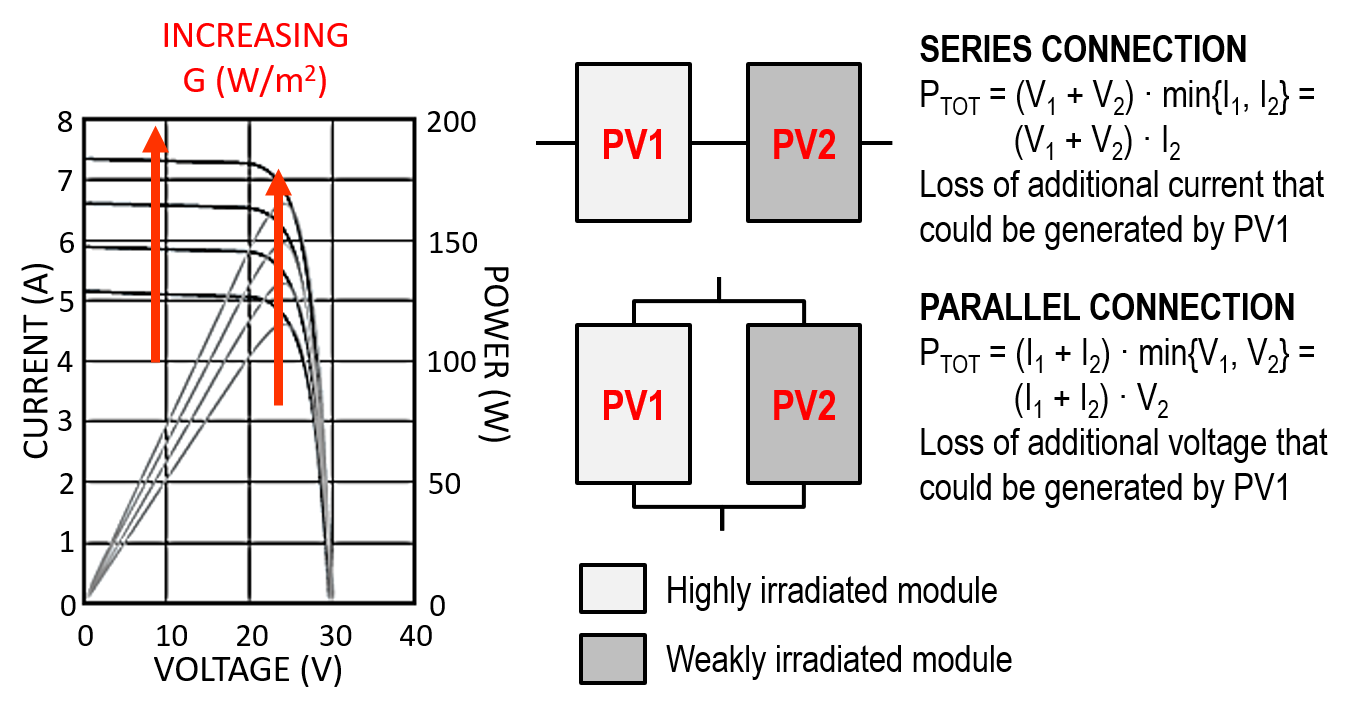
\includegraphics[width=\linewidth]{images/pv_background.png}\vspace{-0.3cm}
\caption{Typical voltage-current (I-V, black) and voltage-power (P-V, gray) curves of a PV module \cite{datasheet} (left), and impact of partial shading on the series or parallel connection of PV modules (right).
}
%\vspace{-0.5 cm}
\label{fig:moduleStructure}
\end{figure}

In any PV installation PV modules are typically connected in series or in parallel to achieve the desired voltage and current levels (right of of Figure~\ref{fig:moduleStructure}). %: the typical connection is organized as a number of parallel strings, each composed of the same number of PV modules connected in series. 
If two connected PV modules work with the same input irradiance, then their connection doubles the output power production. However, this is rarely the case, above all in urban areas where obstacles such as chimneys, surrounding buildings, trees, etc project shadows and determine a heterogeneous distribution of irradiance \cite{LI2020118795}. 
%\subsection{Impact of partial shading on PV production}\label{sec:back_pv:shading}
%In urban areas,\cite{LI202 0118795}. 
%PV installations are typically designed by assuming that the surface of interest is subject to even irradiance. This is however not accurate, as shadows projected by obstacles such as chimneys, surrounding buildings, trees, etc determine a heterogeneous distribution of irradiance, with the effect that each PV module will operate at different irradiance conditions. 

Shading is critical for PV installations, as the least irradiated PV module acts as a bottleneck on power production: the higher the variance of irradiance, the higher the power loss (right of of Figure~\ref{fig:moduleStructure}). 
When PV modules are connected in series, the least irradiated module will provide the smallest current; when PV modules are connected in parallel, the PV module with lowest voltage will determine the voltage of all connected PV modules. 
%This leads to a potentially high power dissipation, resulting in local overheating,  accelerated ageing and permanent cell damage \cite{6528850}. 

